\documentclass{article}
\usepackage{doc,url,verbatim,fancyvrb}
\usepackage{pifont}
\usepackage[authoryear]{natbib}
\usepackage[pdftex]{graphicx}
\usepackage{gretl}
\usepackage[letterpaper,body={6.3in,9.15in},top=.8in,left=1.1in]{geometry}
%\usepackage[pdftex,hyperfootnotes=false]{hyperref}

%\usepackage[a4paper,body={6.1in,9.7in},top=.8in,left=1.1in]{geometry}

\begin{document}

\setlength{\parindent}{0pt}
\setlength{\parskip}{1ex}

\newcommand{\argname}[1]{\textsl{#1}}

\title{ivpanel version 0.5}
\author{Allin Cottrell}
\date{October 19, 2015}
\maketitle

\section{Introduction}

This package estimates three variants of panel data models with
instrumental variables, namely fixed-effects, the ``between'' model,
and random effects (Generalized 2-Stage Least Squares or G2SLS). An
extended discussion of these models can be found in chapter 7 of
\cite{baltagi05}. The sample script provided with this package
replicates results obtained by Baltagi using \textsf{Stata} for
each of the three supported models.

The required arguments to the main public function \texttt{ivpanel()}
are as follows:

\begin{enumerate}
\item \argname{y} (series), the dependent variable
\item \argname{X} (list), the regressors, both exogenous and endogenous
\item \argname{Z} (list), the instruments, including any exogenous
  regressors
\end{enumerate}

Note that exogenous variables in list \argname{X} should be repeated
in \argname{Z}, as in gretl's \texttt{tsls} command. The constant is
automatically added to \argname{X} and \argname{Z} if it's not already
present.

An optional fourth argument, \argname{case}, can be used to specify
the type of model. The argument is an integer switch that takes values
1, 2 or 3 (this may be extended in future).  A value of 1 means fixed
effects, and is implicit if no fourth argument is given; a value of 2
means to use the between estimator; and a value of 3 means G2SLS.
Leaving aside the constant, all the members of \argname{X} and
\argname{Z} must be time-varying when the fixed effects case is
selected.

An optional final boolean argument, \argname{quiet}, controls the
printing of output: if \argname{quiet} is set to a non-zero value,
printing is suppressed.

\section{The ivpanel bundle}

By way of return value, \texttt{ivpanel()} offers a gretl bundle
containing the items shown in Table~\ref{tab:bun}.

\begin{table}[htbp]
\centering
\begin{tabular}{llp{.6\textwidth}}
  \textit{name}   & \textit{type} & \textit{description} \\[4pt]
  \texttt{case}   & scalar & the value of the \argname{case} argument on input \\
  \texttt{nobs}   & scalar & the total number of observations used \\
  \texttt{coeff}  & matrix & column vector of coefficients \\
  \texttt{stderr} & matrix & column vector of standard errors \\
  \texttt{vcv}    & matrix & the coefficient covariance matrix \\
  \texttt{uhat}   & matrix & the vector of residuals \\
  \texttt{yhat}   & matrix & the vector of fitted values \\
  \texttt{SSR}    & scalar & sum of squared residuals \\
  \texttt{sigma}  & scalar & standard error of the regression \\
  \texttt{df}     & scalar & degrees of the freedom for the regression \\
  \texttt{rsq}    & scalar & correlation-based $R^2$  \\
  \texttt{wald}   & scalar & Wald joint $\chi^2$ test for all regressors \\
  \texttt{modstr} & string & short description of the model \\
  \texttt{ystr}   & string & the name of the dependent variable \\
  \texttt{Estr}   & string & the names of the endogenous regressor(s) \\
  \texttt{Istr}   & string & the names of the (additional) instruments \\
  \texttt{dims}   & matrix & data dimensions (cases 1 and 3 only) \\
  \texttt{Fpool}  & scalar & $F$-test for joint significance of fixed
                             effects (case 1 only)
\end{tabular}
\caption{Items in ivpanel bundle}
\label{tab:bun}
\end{table}

Some comments on the bundle members follow.

\begin{itemize}

\item The $R^2$ value, \texttt{rsq}, is calculated as the square of the
  correlation between the dependent variable and the fitted values.

\item The \texttt{dims} vector, if present, contains three elements
  holding, respectively, the number of groups used and the minimum and
  maximum time-series spans.

\item The \texttt{Fpool} statistic for fixed effects is calculated as
  per \cite{wooldridge90}, adjusted for the panel case. The formula is
\[
 \frac{\mbox{SSRr} - \mbox{SSRu}}{\mbox{SSRf}} \times 
  \frac{\mbox{dfd}}{\mbox{dfn}}
\]

 where SSRf is the sum of squared residuals from the fixed-effects IV
 model and the other two SSR values are calculated thus:
\begin{enumerate}
\item We run the fixed-effects first-stage regressions and save the
  fitted values; we then use these to replace the endogenous
  regressors.
\item SSRr is then obtained via OLS, and SSRu from a fixed-effects
  regression. SSRu differs from SSRf in that it uses the ``raw''
  residuals, without correction as one usually applies with two stage
  least squares (i.e.\ replacing the first-stage fitted values with
  the actual data for the endogenous regressors when computing the
  fitted values).
\end{enumerate}

\end{itemize}

\section{Sample script}

The sample script estimates three models of the (log) crime rate
across the counties of North Carolina over the years 1981 to 1987,
using data from \cite{cornwell94}. The endogenous regressors are
\texttt{lpolpc} (log of police per capita) and \texttt{lprbarr} (log
of the estimated probability of arrest). The instruments (besides the
exogenous regressors) are \texttt{ltaxpc} (log of tax revenue per
capita), \texttt{lmix} (log of the offense ``mix'', face-to-face
versus other) and a set of year dummies. 

It's perhaps noteworthy that despite the IV approach, the coefficient
on \texttt{lpolpc} is positive in all the models, the opposite of what
would be expected if the estimator had succeeded in picking up a
causal relationship. At least in the fixed effects specification the
positive \texttt{lpolpc} coefficient is not statistically significant
($P$-value > 0.4).

\section{Graphical interface}

An entry-point for \textsf{ivpanel} can be found under the
\textsf{Panel} sub-menu of gretl's \textsf{Model} menu: the label is
``Panel IV model.'' See Figure~\ref{fig:gui}. The specification of the
endogenous regressors is implicit: any variables that appear in the
``regressors'' list and not in the ``instruments'' list are taken to
be endogenous.

\begin{figure}[htbp]
  \centering
  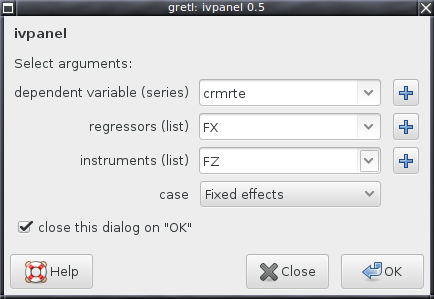
\includegraphics[scale=0.6]{ivpanel-gui}
  \caption{Specify arguments for ivpanel}
  \label{fig:gui}
\end{figure}

\section{Auxiliary printing function}

The auxiliary public function \texttt{ivp\_print()} is provided to
``pretty-print'' the results contained in the bundle provided by
\texttt{ivpanel()}; \texttt{ivp\_print()} takes a pointer to the
bundle as its sole argument.

\bibliographystyle{gretl}
\bibliography{gretl}

\end{document}
